%Thomas
\newpage
\usecase{Besucher sucht einen ehemaligen Kommilitonen}
\usecasepart{Anmeldung am Alumni-Portal}

\subsubsection*{Positive Beobachtungen}
Das Anmeldeformular für das Portal ist an einer zentralen und gut einsehbaren Stelle positioniert. Dadurch ist es direkt im Blickfeld des Nutzer und kann jederzeit seine Verwendung finden. Zwei Eingabefelder ermöglichen das Eintippen der Zugangsdaten, mit denen sich der Benutzer am Portal authentifizieren kann. Unklarheiten bezüglich der einzugebenden Daten entstehen durch die klare Struktur und die Beschriftung der Elemente nicht. Der Button \emph{Anmelden} führt wie erwartet den Login aus. Abschließend ist positiv anzumerken, dass nach Absenden des Formulars der Benutzer visuelles Feedback eingeblendet bekommt. Dadurch wird veranschaulicht, dass das System die Anfrage zum Login bearbeitet.

\problem{Dezentes Feedback bei fehlerhaftem Login}
{
	Erfolgt eine fehlerhafte Eingabe von Benutzername und Passwort durchläuft das System den kompletten Vorgang der Anmeldung. Die Login-Daten werden verarbeitet und abschließend wird die Portalseite neu geladen. Befindet sich der Nutzer zum Zeitpunkt des Login nicht auf der Startseite, so wird er dorthin weitergeleitet. Die neu aufgebaute Startseite blendet dem Nutzer Feedback in Form eines kurzen Hinweistextes ein. Dieser teilt mit, dass aufgrund ungültiger Zugangsdaten die Authentifizierung nicht möglich war. Die Platzierung sowie Formatierung des Feedback ist sehr schlicht und unauffällig gewählt. Unerfahrene Anwender übersehen eine derartige Fehlermeldung unter Umständen und warten auf eine Reaktion von Seiten des Systems.
}
{
	Das aufgeführte Problem ist nicht derart schwerwiegend, als dass es die Funktionalität der Seite in irgendeiner Form einschränkt. Durch verminderte Aufmerksamkeit des Anwenders kann es jedoch dazu führen, dass wichtiges Feedback schlichtweg nicht wahrgenommen wird. Somit ist die Art und Weise der Rückmeldung von Webseite an Benutzer nicht auffällig genug gestaltet. Aus den genannten Gründen lassen sich diese Umstände der Kategorie als \emph{mittelschweres Problem} zuordnen (Kategorie 2).		
}
{
	Ziel ist es, dass der Nutzer eingeblendetes Feedback, welches vom System erzeugt wird, auffällig und gut sichtbar präsentiert bekommt. Deshalb empfiehlt sich eine entsprechende Farbgestaltung: rot für Fehlermeldungen, gelb für Warnungen und grün für erfolgreich durchgeführte Aktionen. Weiterhin ist die Schriftgröße angemessen zu wählen. Eine einheitliche Platzierung des Feedback ist ebenso erstrebenswert. Bei Eingabefeldern ist es beispielsweise empfehlenswert fehlerhafte Eingaben und dazugehörige Hinweistexte in unmittelbarer Nähe des betroffenen Elements zu platzieren.
}
\label{prob:suche:loginfehler}


% Aufgabenteil
% ------------
\usecasepart{Aufrufen der Suchmaske über das Menü}

\subsubsection*{Positive Beobachtungen}
Das horizontal angelegte Menü unterhalb der Headergrafik ist schlicht und übersichtlich gehalten. Die darin aufgelisteten Menüpunkte sind eindeutig und leicht verständlich beschrieben. Weiterhin lässt deren Benennung einen direkten Rückschluss darauf zu, welche Funktionalität der Benutzer dahinter zu erwarten hat. So ist beispielsweise direkt ersichtlich, dass sich hinter dem Punkt \emph{Alumni suchen} im Menü eine Suchmaske befindet.

\problem{Suchanfrage startet unverzüglich nach Seitenaufbau}
{
	Nach einem Klick auf \emph{Alumni suchen} im Menü öffnet sich direkt die Suchmaske zur Eingabe von Kontaktdaten. Zu diesem Zeitpunkt ist das Suchfeld vom Anwender unberührt: es erfolgte bisher keine Eingabe. Nach dem erfolgreichen Seitenaufbau startet unaufgefordert der Suchvorgang mit einem leeren Suchbegriff. Als Ergebnis vermeldet das System, dass keine passenden Datensätze zu der Suche vorhanden sind. Dem Benutzer werden zusätzlich Elemente zur Navigation (vorwärts und rückwärts blättern) innerhalb der Trefferliste angezeigt. Das Ausführen der Funktionalität der beschriebenen Navigationselemente ist bei leerem Ergebnis nicht möglich.
}
{
	Das sofortige starten eines Suchvorgang trotz fehlender Eingabe wirkt deplatziert und ist überflüssig. Die eingeblendeten Elemente für das Blättern in der Ergebnisliste bieten dem Anwender ebenfalls kein Mehrwert. Bedienung und Funktionalität der Webseite sind aufgrund des beschriebenen Sachverhaltes nicht eingeschränkt. Hierbei handelt es sich um ein \emph{mittelschweres Problem} (Kategorie 2).
}
{
	Das Auslösen der Suche nach dem vollständigen Aufbau der Seite entfernen. Dadurch lässt sich sowohl die Ladezeit des Inhaltes, als auch eine überflüssige Abfrage an die Datenbank einsparen. Weiterhin sollten dem Nutzer keine überflüssigen Funktionselemente angezeigt werden, für die er zum derzeitigen Zeitpunkt keine Verwendung findet.
}
\label{prob:suche:suchanfrage}

% Aufgabenteil
% ------------
\usecasepart{Auswahl der gewünschten Suchmaske}
%\subsubsection*{Positive Beobachtungen}
%... 

\problem{Seitenmenü unübersichtlich/inkonsistent gestaltet}
{
	Im linken Bereich auf der Unterseite \emph{Alumni suchen} befindet sich ein zusätzliches Menü, über welches der Nutzer die Eingabemaske für die Suche wechseln kann. Zur Veranschaulichung dient die Abbildung \ref{fig:suche:seitlichesmenue}. Die Visualisierung der vertikal angelegten Menüelemente (Farbe und Formatierung) ist unüblich gewählt. Es ist nicht eindeutig erkennbar, welcher Menüpunkt als aktiv gesetzt ist. Dem Anwender fehlt somit das Verständnis, welche Suchmaske ihm aktuell angezeigt wird. Bekannte Mouse-Over Effekte bei Hyperlink-Elementen finden in der Menüleiste keine Verwendung. Die dort eingesetzte Farbe Schwarz in einem Navigationselement ist ebenfalls von Nachteil. Für gewöhnlich gehen Nutzer bei dieser Formatierung von normalen Textelementen aus und erwarten nicht einen Link zum Klicken.
	\begin{figure}[h]
		\centering
		
\includegraphics[scale=0.75]{figures/seitliches_menue.png}
		\caption{Seitenmenü bei der Suche nach einem Alumni}
		\label{fig:suche:seitlichesmenue}
	\end{figure}
}
{
	Die ungewöhnliche Wahl der Formatierung für Hyperlinks und die fehlende Hervorhebung des aktiv gewählten Menüelements sorgt beim Endanwender für Verwirrung. Dies wiederum führt zur falschen Verwendung der im Menü angebotenen Aktionen. Aufgrund dieser Umstände lässt sich das Problem in die Kategorie \emph{mittelschweres Problem} einstufen. Die Funktionalität der Webseite ist hierdurch nicht eingeschränkt (Kategorie 2).
}
{
	Das seitliche Menü im unmittelbaren Blickfeld des Anwender platzieren. Hierfür bietet sich die Positionierung als zusätzliche horizontale Navigation im Inhaltsbereich der Suchseite an. Dadurch wird die Aufmerksamkeit des Nutzers angezogen und die Existenz der unterschiedlichen Eingabemasken hervorgehoben. Zudem empfiehlt sich die Formatierung von Hyperlink-Elementen an die Gewohnheiten erfahrener Nutzer anzupassen: unterstreichen, eine eigene Farbe für Links und einen angemessenen Mouse-Over Effekt dieser Elemente.
}
\label{prob:suche:seitenmenue}

% Aufgabenteilgit p
% ------------
\usecasepart{Alumni über einen Suchbegriff finden}
%\subsubsection*{Positive Beobachtungen}
%... 

\problem{Suchvorgang mit fehlender Eingabe ausführbar}
{
	Eine Eingabe in die Suchmaske ist nicht zwingend erforderlich. Dem Anwender wird gestattet einen Suchvorgang mit leerer Eingabe zu starten. Nach einem Neuaufbau der Seite wird ein visuelles Feedback eingeblendet, das darauf hinweist, dass mindestens ein Suchbegriff notwendig ist. Trotz gescheiterter Suche wird wiederum eine leere, nicht benötigte Trefferliste mit dazugehörigen Elementen zur Navigation angezeigt.
}
{
	Das beschriebene Probleme schränkt den Anwender der Webseite hinsichtlich Bedienung und Funktionalität nicht ein. Die Tatsache, dass eine leere Suche nicht im Vorfeld bereits von Seiten des System unterbunden wird, kann beim Benutzer jedoch auf Unverständnis treffen. Insgesamt lässt sich dieser Umstand als \emph{mittelschweres Problem} einstufen (Kategorie 2).
}
{
	Eine denkbare Lösung ist es, den Button zum Starten der Suche so lange zu deaktivieren, bis der Endanwender mindestens ein Suchbegriff/-wort eingegeben hat. Danach kann der Suchvorgang wie gewohnt über den danebenliegenden Button gestartet werden. Ein alternativer Verbesserungsvorschlag ist es, dem Nutzer unmittelbar Feedback zu präsentieren und ihn auf das Fehlen eines Suchbegriffs hinzuweisen. Dadurch wird ein unnötiges Neuladen der Webseite verhindert, sowie die damit verbundenen Wartezeit während die Seite sich aktualisiert.
}
\label{prob:suche:leereeingabe}

\problem{Keine eindeutige Festlegung für Eingabe in das Suchfeld}
{
	Bei der Suche nach einem Alumni anhand von Kontaktdaten ist die Eingabe in das vorgesehene Feld nicht eindeutig festgelegt. Intuitiv geht der Nutzer davon aus, dass er den Namen der zu suchenden Person in das Eingabefeld eingeben soll. Bei einem ausführlichen Test wird ersichtlich, dass alle personenbezogenen Daten Gegenstand einer Suchenanfrage sein können. Darunter fällt beispielhaft der Wohnort, der Straßenname, die E-Mail Adresse, sowie derzeitige Tätigkeit und Firma in der die Person arbeitet.
}
{
	Die Suche funktioniert auf den ersten Blick so wie es der Nutzer erwartet. Ein Suchbegriff wird eingegeben und daraufhin werden alle Ergebnisse eingeblendet, die eben diesen String  beinhalten. Da nicht kommuniziert wird, welche Eingabe vom Anwender erwartet wird, ist nicht eindeutig vorhersehbar, mit welchen persönlichen Daten der Alumni die Sucheingabe abgeglichen wird. Der Umstand einer fehlenden Information hinsichtlich zu tätigender Eingabe lässt dieses Problem der Katgorie \emph{mittelschweres Problem} zuordnen (Kategorie 2).
}
{
	Da die Webseite dem Benutzer eine erweiterte Suchfunktionalität anbietet, ist es denkbar die grundlegende Sucheingabe auf den Vor- und Nachnamen der zu suchenden Person zu beschränken. Ein erklärender Hinweis für den Benutzer hinsichtlich gültiger Eingabewerte ist notwendig. Eine Suche mit spezifischen Angaben zur Person sollte künftig über die erweiterten Suchoptionen getätigt werden.
}
\label{prob:suche:eingabeuneindeutig}

\problem{Anzeige der Trefferanzahl während Sucheingabe}
{
	Tippt der Nutzer einen Suchbegriff ein, so wird umgehend eine Abfrage an die Datenbank gesendet, welche die Anzahl an Treffern zu dieser Eingabe zurückliefert. Erkenntlich ist dies an der Lade-Animation rechts neben dem Eingabefeld, wo nach erfolgreicher Abfrage das Resultat angezeigt wird. Diese Funktionalität bietet dem Anwender zum genannten Zeitpunkt der Eingabe keinerlei wertvollen Informationsgehalt. Zumal der Suchvorgang explizit über den Button \emph{Suchen} gestartet werden muss bevor eine Trefferliste angezeigt wird. Das eingeblendete Ladesymbol kann den Endanwender zusätzlich verwirren, der die Eingabe unter Umständen noch nicht beendet hat. Das System vermittelt jedoch den Eindruck, als würde die Suchabfrage bereits durchgeführt werden.}
{
	Das unmittelbar während der Eingabe erscheinende Ladesymbol und die noch nicht abgeschickte Suche können den Nutzer aus dem Konzept bringen. Zudem ist die Position, sowie die Art des Feedbacks zum Zeitpunkt der Eingabe für den Nutzer in dieser Art und Weise wertlos. Hierbei handelt es sich bereits um ein \emph{schweres Problem} (Kategorie 3).
}
{
	Zum Zeitpunkt der Eingabe kann der Nutzer sehr gut auf die Anzahl der Treffer mit dem eben eingetippten Suchbegriff verzichten. Aus diesem Grund sollte die zudem wenig aussagekräftige Information vollständig weggelassen werden. Durchaus interessanter --- und vom Informationsgehalt wertvoller --- dürfte eine Autovervollständigung sein. Diese schlägt dem Nutzer während der Eingabe mögliche Vervollständigungen vor, die aufgrund des bereits eingegebenen String und dem Datenbestand der Alumni Benutzerliste getroffen werden können.
} 
\label{prob:suche:trefferanzeige}

\problem{Suchvorgang durchsucht alle Datenfelder}
{
	Im vorherigen Verlauf des Walkthrough ist das Problem beschrieben, dass die Sucheingabe nicht eindeutig festgelegt ist. Betrachten wir im Anschluss nun die Ergebnisliste einer Suche genauer. Es fällt auf, dass Treffer aufgelistet sind, die aufgrund der Eingabe für den Suchenden nicht relevant sind. Bei dem Betrachten der Profilseite der nicht relevanten Treffer wird ersichtlich, dass alle Angaben zur Person mit dem eingegebenen Begriff abgeglichen werden. So findet das Portal bei dem Suchstring \glqq .de\grqq ~alle Nutzer, die sich mit einer .de E-Mail-Adresse angemeldet haben. Ein weiteres Beispiel: die Anschrift eines Alumni beinhaltet einen Vornamen (z.B. Anna-Straße 24).
}
{
	Aus Sicht des Nutzers arbeitet die Suchfunktion nicht nach den eigenen Vorstellungen und führt die Aktion fehlerhaft aus. Intuitiv geht der Endanwender davon aus, dass mit der normalen Suchfunktion vorrangig nach dem Namen eines Alumni gesucht werden kann. Tauchen in der Trefferliste Personen auf, deren Namen komplett von der Eingabe abweichen, so stößt dies auf Unverständnis und verwirrt den Nutzer. Bei dieser fehlerhaften und unerwarteten Funktionalität handelt es sich um ein \emph{fatales Problem} (Kategorie 4).
}
{
	Bei der Sucheingabe muss festgelegt sein, welche Eingaben dem Nutzer gestattet sind und dadurch ersichtlich werden, welche Ergebnisse zu erwarten sind. Im vorliegenden Szenario ist es sinnvoll die normale Suche lediglich auf den Namen zu beschränken und dies im Eingabefeld per \glqq Hint\grqq ~vorzugeben. Für eine detaillierte Suche steht dem Suchenden zudem ein entsprechendes Formular mit erweiterten Eingabemöglichkeiten zur Verfügung. Mit Hilfe von diesem ist es ihm gestattet seine Suche weiter zu verfeinern.
} 
\label{prob:suche:sucheallefelder}

% Aufgabenteil
% ------------
\usecasepart{Alumni über erweiterte Suchoptionen finden}

\subsubsection*{Positive Beobachtungen}
Das ausgeklappte, erweiterte Suchmenü wirkt auf den Benutzer ordentlich gegliedert und auf den ersten Blick aufgeräumt. Die zu tätigenden Eingaben sind nach Obergruppen (private und geschäftl. Kontaktdaten) strukturiert und beinhalten die zugehörigen Eingabefelder.

\problem{Zu viele Eingabefelder für den Nutzer}
{
	Die Eingabefelder sind gruppiert und wirken auf den ersten Blick aufgeräumt. Bei näherem Betrachten fällt jedoch der hohe Detailgrad auf, mit dem die Suche ausgefüllt werden kann. Viele der anzugebenden Informationen stehen dem Suchenden im Regelfall nicht zur Verfügung und sind unbekannt. Durch diese Umstände wirkt die Eingabemaske unnötig überladen.
}
{
	Die Funktionalität der Webseite sowie die Suchfunktion sind aufgrund der Fülle an Eingabemöglichkeiten in keinster Weise eingeschränkt. Eine derart umfangreiche Suchmaske schreckt den Benutzer oftmals vor dem Ausfüllen ab. Es handelt sich um ein \emph{leichtes Problem} (Kategorie 1).
}
{
	Um dem Benutzer eine komfortable und schnelle Eingabe erweiterter Suchoptionen zu ermöglichen, bietet es sich an diese stark zu reduzieren. Dazu können überflüssige, bzw. zu detaillierte Formularfelder, bezüglich Werdegang und geschäftlichen Kontaktdaten, herausgenommen werden. Es macht wenig Sinn anhand zu spezifischer Kriterien eine Suche nach ehemaligen Kommilitonen/Alumni-Mitgliedern zu starten.
}
\label{prob:suche:vieleeingabefelder}

\problem{Speichern/Laden der Suche nicht implementiert}
{
	Dem Anwender wird am Fuß der erweiterten Suchmaske die Funktionalität angeboten, das ausgefüllte Formular zu speichern und bei späteren Suchanfragen wieder zu verwenden. Das Gegenstück hierzu --- eine zuvor ausgefüllte Suche laden --- ist ebenfalls über einen Hyperlink erreichbar. Nach Klick auf \emph{Suche speichern} wird der Anwender aufgefordert eine Bezeichnung für die ausgefüllte Suche zu vergeben (siehe Abb. \ref{fig:suche:speichern}). Hinter dem Button \emph{Speichern}, um die Eingabe zu persistieren, verbirgt sich jedoch keine Funktionalität. Das Abspeichern der Suchmaske ist beim derzeitigen Stand der Webseite nicht implementiert. Umgekehrt ist das Laden einer zuvor gespeicherten Suche nicht durchführbar, da die Funktionalität \emph{Suche speichern} nicht verwendbar ist.
	\begin{figure}[h]
		\centering
		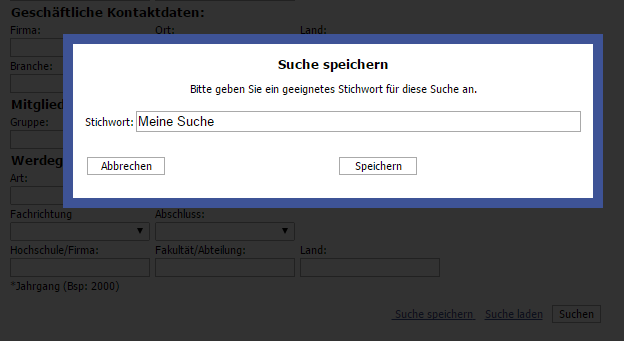
\includegraphics[scale=0.75]{figures/suche_speichern.png}
		\caption{Dialog für das Speichern einer Suchmaske}
		\label{fig:suche:speichern}
	\end{figure}
}
{
	Bei der beschriebenen Situation handelt es sich um einen klaren \glqq Showstopper\grqq . Dem Benutzer wird eine Funktionalität zur Verfügung gestellt, die allerdings nicht die erwartete Aktion ausführt. Sie bewirkt keinerlei Aktion. Aus diesem Grund handelt es sich um ein \emph{fatales Problem}, das den Anwender hinsichtlich angebotener Funktionalität der Webseite einschränkt (Kategorie 4).
}
{
	Eine Möglichkeit besteht darin, das Abspeichern der Suchmaske zu implementieren. Dadurch erhält der Benutzer die zuvor beschriebene Funktionalität geboten und kann diese wie erwartet einsetzen. Alternativ kann die Funktion \emph{Suche speichern} komplett von der Webseite entfernt werden. Es ist eher ungewöhnlich das Speichern einer Suchmaske anzubieten. Ein sinnvoller Anwendungsfall tritt nur selten auf und die Funktionalität bietet geringen Mehrwert für den Nutzer des Systems.
}
\label{prob:suche:suchespeichern}

% Aufgabenteil
% ------------
\usecasepart{Alumni über die Studiengangliste finden}

\subsubsection*{Positive Beobachtungen}
Durch die große Anzahl verschiedener Studiengänge wird die daraus resultierende Liste sehr lang. Mit Hilfe der bereitgestellten Filter wird dem Anwender ein hilfreiches Werkzeug an die Hand gegeben, um den Umfang der Auflistung stark zu reduzieren. Dies ist ihm sowohl anhand des Anfangsbuchstaben gestattet, als auch in Form einer Jahreszahl für Beginn sowie Ende der Studienzeit. 

\problem{Fehlendes Feedback beim Laden der Studiengangsliste}
{
	Entscheidet sich der Nutzer einen Alumni anhand des Studiengangs zu suchen, so nutzt er die Suchfunktion hinter dem Menüpunkt \emph{Studiengangs-/Jahrgangsliste} in der linken Navigation. Nach dem Klick präsentiert sich dem Anwender zunächst ein leerer Inhaltsbereich. Zu diesem Zeitpunkt meldet das System kein Feedback an den Nutzer. Es ist in dieser Situation nicht ersichtlich, ob der Ladevorgang abgeschlossen, abgebrochen oder noch in Arbeit ist. Der Benutzer erhält den Eindruck als befände er sich auf einer Unterseite ohne entsprechenden Inhalt. Erst nach längerer Wartezeit erscheint die Liste aller Studiengänge.
}
{
	Das System berichtet dem Anwender nicht den aktuellen Zustand der Aktion. Es ist nicht ersichtlich, ob in absehbarer Zeit die Aktion beendet und der erwartete Inhalt angezeigt wird. Die beschriebene Thematik lässt sich als \emph{fatales Problem} einstufen (Kategorie 4). Aufgrund des fehlenden Feedbacks vom System wird der Nutzer die Unterseite höchst wahrscheinlich vorzeitig verlassen. 
}
{
	Abhilfe schafft das Anzeigen von Feedback für den Nutzer. Die einfachste Möglichkeit hierfür ist eine Animation in Form eines Ladebalken oder “Spinner”, die dem wartenden Benutzer angezeigt wird. Dadurch wird signalisiert, dass das System im Hintergrund noch arbeitet und in absehbarer Zeit das Ergebnis präsentiert wird.
}
\label{prob:suche:keinfeedback}

\problem{Unübersichtliche Darstellung der Studiengangsliste}
{
	Die Liste, welche alle eingetragenen Studiengänge beinhaltet, erstreckt sich über eine Spalte und kann entsprechend sehr lang werden. Durch die relativ kurzen Bezeichnungen der Studiengänge wird die Breite des Inhaltsbereichs nicht vollständig ausgeschöpft. Es wird vom Nutzer erwartet, dass er entsprechend weit auf der Webseite nach unten scrollt. Nur so ist es ihm gestattet, alle Einträge der Liste sehen zu können.
}
{
	Bei dieser Problembeschreibung handelt es sich lediglich um geringe Mängel am User-Interface. Es sind dadurch keinerlei Einschränkungen der Funktionalität gegeben. Die Umstände lassen sich als \emph{leichtes Problem} einordnen (Kategorie 1).
}
{
	An dieser Stelle bietet sich ein mehrspaltiges Layout für die Liste aller Studiengänge an. Hiermit wird der Inhaltsbereich besser ausgenutzt und es entsteht beim Anwender nicht der Eindruck einer unendlichen Auflistung. Die Studiengänge lassen sich somit viel schneller auffassen ohne auf der Webseite weit nach unten scrollen zu müssen.
}
\label{prob:suche:studiengangsliste}

\problem{Ungültige Studiengänge erscheinen in der Liste}
{
	In der Studiengangliste sind zum Teil fehlerhafte und mit Rechtschreibfehlern behaftete Studiengänge aufgelistet. Diese entstehen unter anderem bei der Registrierung durch einen neuen Benutzer am Alumni-Portal. Das Anmeldeformular gestattet bei der Registrierung die Eingabe von individuellen Studiengängen, wodurch fehlerhafte Eingaben entstehen können.
}
{
	Aufgrund des falsch zugeordneten Studiengangs im Profil eines Alumni ist es durchaus möglich, dass der Benutzer das gewünschte Mitglied nicht finden kann. Somit ist das Ziel dieses Use-Case theoretisch nicht erreichbar. Es handelt sich um ein \emph{schweres Problem} (Kategorie 3).
}
{
	Derartige Fehleingaben bei der Registrierung lassen sich durch eine Validierung der Eingabedaten des entsprechenden Formulars verhindern. Dieser Lösungsvorschlag ist jedoch nicht Bestandteil von diesem Use-Case, sondern wird in Kapitel \ref{usecse:reg} (\nameref{usecse:reg}) ausführlich behandelt.
}
\label{prob:suche:ungueltigestudiengaenge}

% Aufgabenteil
% ------------
\usecasepart{Sichten der Trefferliste einer Suche}

\subsubsection*{Positive Beobachtungen}
Die Trefferliste ist übersichtlich und gut strukturiert aufgebaut. Die einzelnen Resultate heben sich mit Hilfe unterschiedlicher Hintergrundfarben gut voneinander ab. Zudem erhält der Endanwender direkt in der Ergebnisliste die ersten wichtigen Informationen zu den Personen, wie der aktuelle Wohnort, ein Profilbild (sofern vorhanden) und den vollständigen Namen. Weiterhin positiv anzumerken sind die Blätter-Elemente mit deren Hilfe der Anwender durch die gesamte Ergebnisliste navigieren kann. Dabei stehen ihm folgende Funktionen zur Verfügung: vorwärts und rückwärts blättern, sowie an den Anfang bzw. das Ende der Trefferliste springen. 

\problem{Hinweis \glqq Unbekannter Typ\grqq ~bei Suchtreffern}
{
	In der Liste aller Treffer erscheint bei einzelnen Resultaten der Hinweistext \glqq Unbekannter Typ\grqq ~in rot und fett gedruckter Schrift (siehe Abb. \ref{fig:suche:unbekanntertyp}). Dieser ist zurück zu führen auf eine  fehlende Eingabe im persönlichen Profil des betroffenen Alumni. Dieser Hinweistext hat für den Anwender keinerlei Informationsgehalt und trägt viel mehr zur Verwirrung bei. Der Grund für diesen auffällig gestalteten Text ist für den Suchenden nicht ersichtlich. Die Aufmerksamkeit des Nutzers wird unnötigerweise auf diesen Hinweis gezogen.
	\begin{figure}[h]
		\centering
		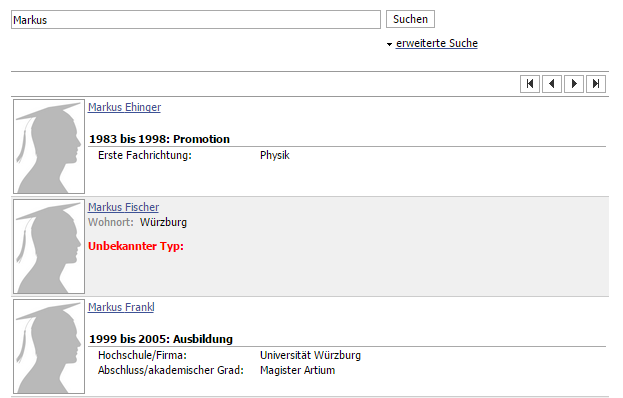
\includegraphics[scale=0.75]{figures/unbekannter_typ.png}
		\caption{Ergebnisliste mit Treffer \glqq Unbekannter Typ\grqq}
		\label{fig:suche:unbekanntertyp}
	\end{figure}
}
{
	 Die eingeblendete Profilinformation ist für den Benutzer nicht nachvollziehbar, schränkt die Funktionalität der Webseite allerdings nicht ein. Aus diesem Grund ist diese Auffälligkeit lediglich der Kategorie \emph{mittelschweres Problem} zuzuordnen (Kategorie 2).
}
{
	Handelt es sich um eine fehlende Eingabe von Seiten des entsprechenden Alumni kann dieser Hinweistext ebenso gut ausgeblendet und nicht präsent sein. Dadurch stellt sich dem Suchenden nicht die Frage, welche Informationen damit verbunden sind. Eine alternative Verbesserung ist es die Meldung mit mehr Informationsgehalt auszustatten, so dass der Benutzer versteht, wieso an dieser Stelle ein auffälliger Hinweistext angezeigt wird.
}
\label{prob:suche:unbekanntertyp}

\problem{Trefferanzahl pro Seite und Blätterfunktion}
{
	Bei den Suchergebnissen ist die Anzahl der Treffer fest auf fünf pro Seite festgelegt. Dadurch ist der Anwender gezwungen sehr oft zu blättern, sofern sich der gesuchte Alumni mindestens in der zweiten Hälfte der Liste befindet. Dabei wird auch die eingeschränkte Funktionalität ersichtlich, zwischen den Seiten der Ergebnisliste hin und her zu springen. Es ist dem Anwender nur gestattet eine Seite vor- bzw rückwärts zu blättern, bzw. direkt an den Anfang/das Ende der Trefferliste zu springen. Die Bedienung der Blätterfunktion ist somit aus Sicht des Nutzers stark eingeschränkt und gestaltet die Bedienung ineffizient und unangenehm.
}
{
	Die Funktionalität und Handhabung der Webseite ist durch dieses Problem nicht vollständig eingeschränkt. Durch die festen Vorgaben von Seiten des System (Anzahl Treffer pro Seite, nur eine Seite vor- oder zurückblättern) werden dem Nutzer diesbezüglich keinerlei Freiheiten eingeräumt. Die beschriebene Problematik lässt sich der Kategorie \emph{mittelschweres Problem} zuordnen (Kategorie 2).
}
{
	Die Anzahl der Treffer pro Seite lassen sich variabel gestalten. Der Nutzer kann per Drop-Down Menü selbst bestimmen wie viele Resultate auf einer Seite angezeigt werden sollen. Die Blätterfunktion lässt sich dahingehend verbessern, dass nicht nur ein Vorwärts- und Rückwärts-Button angeboten wird. Das Element zum Navigieren wird hierzu komplett umgestaltet. Wie diese Navigation aussehen kann, verdeutlicht Abb. \ref{fig:suche:pagination}.
	
	\begin{figure}[h]
		\centering
		
\includegraphics[scale=0.75]{figures/pagination.png}
		\caption{Navigationselemente für Ergebnisliste einer Suche}
		\label{fig:suche:pagination}
	\end{figure}
}
\label{prob:suche:trefferanzahl}